%%%%%%%%%%%%%%%%%%%%%%%%%%%%%%%%%%%%%%%%%12pt: grandezza carattere
                                        %a4paper: formato a4
                                        %openright: apre i capitoli a destra
                                        %oneside: solo fronte
                                        %report: stile tesi (oppure book)
\documentclass[12pt,a4paper,openright, oneside]{report}
\usepackage[utf8]{inputenc}

%%%%%%%%%%%%%%%%%%%%%%%%%%%%%%%%%%%%%%%%%libreria per scrivere in italiano
\usepackage[italian]{babel}
\usepackage{listings}
\usepackage{longtable}

%%%%%%%%%%%%%%%%%%%%%%%%%%%%%%%%%%%%%%%%%libreria per accettare i caratteri
                                        %digitati da tastiera come "è" o "à"
\usepackage[T1]{fontenc}
\usepackage[utf8]{inputenc}
\usepackage{comment}

%%%%%%%%%%%%%%%%%%%%%%%%%%%%%%%%%%%%%%%%%libreria per impostare il documento
\usepackage{fancyhdr}
%
%%%%%%%%%%%%%%%%%%%%%%%%%%%%%%%%%%%%%%%%%libreria per avere l'indentazione
%%%%%%%%%%%%%%%%%%%%%%%%%%%%%%%%%%%%%%%%%   all'inizio dei capitoli, ...
\usepackage{indentfirst}

%%%%%%%%%%%%%%%%%%%%%%%%%%%%%%%%%%%%%%%%%libreria per inserire grafici
\usepackage{graphicx}
\usepackage{float}

%%%%%%%%%%%%%%%%%%%%%%%%%%%%%%%%%%%%%%%%%libreria per utilizzare font
                                        %   particolari ad esempio
                                        %   \textsc{}
\usepackage{newlfont}

\oddsidemargin=30pt \evensidemargin=20pt%impostano i margini

%%%%%%%%%%%%%%%%%%%%%%%%serve per la sillabazione: tra parentesi 
					   %vanno inserite come nell'esempio le parole 
					   %che latex non riesce a tagliare nel modo giusto andando a capo.
\hyphenation{sil-la-ba-zio-ne pa-ren-te-si}

%
%%%%%%%%%%%%%%%%%%%%%%%%%%%%%%%%%%%%%%%%%comandi per l'impostazione
                                        %   della pagina, vedi il manuale
                                        %   della libreria fancyhdr
                                        %   per ulteriori delucidazioni
\pagestyle{fancy}\addtolength{\headwidth}{20pt}
\renewcommand{\chaptermark}[1]{\markboth{\thechapter.\ #1}{}}
\renewcommand{\sectionmark}[1]{\markright{\thesection \ #1}{}}
\rhead[\fancyplain{}{\bfseries\leftmark}]{\fancyplain{}{\bfseries\thepage}}
\cfoot{}
%%%%%%%%%%%%%%%%%%%%%%%%%%%%%%%%%%%%%%%%%
\linespread{1.3}                        %comando per impostare l'interlinea
%%%%%%%%%%%%%%%%%%%%%%%%%%%%%%%%%%%%%%%%%definisce nuovi comandi

%%%%%%%%%%%%%%%%%%%%%%%%%%%%%%%%%%%%%%%package per inserire collegamenti ipertestuali.
\usepackage{hyperref}

\begin{document}
\begin{titlepage}
                
%%%%%%%%%%%%%%%%%%%%%%%%%%%%%%%%%%%%%%%%
\clearpage{\pagestyle{empty}\cleardoublepage}%non numera l'ultima pagina sinistra
\end{titlepage}
\pagenumbering{roman}                   %serve per mettere i numeri romani

\chapter*{Introduzione}                 %crea l'introduzione (un capitolo
                                       %   non numerato)
%%%%%%%%%%%%%%%%%%%%%%%%%%%%%%%%%%%%%%%%%imposta l'intestazione di pagina
\rhead[\fancyplain{}{\bfseries
INTRODUZIONE}]{\fancyplain{}{\bfseries\thepage}}
\lhead[\fancyplain{}{\bfseries\thepage}]{\fancyplain{}{\bfseries
INTRODUZIONE}}
%%%%%%%%%%%%%%%%%%%%%%%%%%%%%%%%%%%%%%%%%aggiunge la voce Introduzione
                                        %   nell'indice
\addcontentsline{toc}{chapter}{Introduzione}

La tecnologia Blockchain, introdotta inizialmente come registro distribuito per le transazioni della moneta digitale Bitcoin nel 2008, ha suscitato grande interesse nel corso degli ultimi anni. In poco tempo si è capito come tale tecnologia potesse essere applicata ai campi più disparati, e non soltanto alle monete elettroniche. Fra le tante applicazioni che si prospettano per le blockchain vi sono, ad esempio, il settore energetico, il sistema sanitario, e la tracciabilità delle catene di fornitura di beni, servizi o prodotti alimentari. Il futuro insomma, sembra orientato verso un'adozione delle blockchian su scala globale. Tuttavia, è necessario risolvere una serie di problematiche affinchè ciò possa avvenire. Il difetto forse più importante da questo punto di vista, è che la tecnologia blockchain, per come è stata progettata, non è scalabile. Non sarebbe pertanto capace di supportare un volume di transazioni pari o superiore a quello di circuiti di pagamento globali come Visa o MasterCard, per fare un esempio. Mentre vengono studiate possibili soluzioni per aggirare il problema nelle blockchain esistenti, sono nate piattaforme alternative alle blockchain che promettono una maggiore scalabilità, nonchè facilità nel costruire applicazioni basate su esse. E' il caso di Radix DLT. In questa tesi ho deciso di concentrarmi su Radix DLT e di realizzare una piccola applicazione per provare con mano gli strumenti di sviluppo a disposizione. 

La tesi è strutturata come segue:
\begin{itemize}

    \item Nel primo capitolo si presenta una breve panoramica sulla storia e sulle caratteristche principali della tecnologia blockchain. In particolare si parlerà di Bitcoin come punto di partenza della blockchain delle, e successivamente dell'arrivo di Ethereum, con la blockchain non più applicabile esclusivamente al campo delle criptovalute, ma come base per lo sviluppo di applicazioni decentralizzate, dette DApps, per i compiti più disparati. Si evidenzierà poi come le blockchain presentano problematiche che ne impediscono un'adozione su scala globale, e in particolar modo ci si concentrerà sulla mancanza di scalabilità di esse. Infine, si presenterà la piattaforma Radix DLT, un'alternativa scalabile alle blockchain classiche.
    
    \item Nel secondo capitolo si presenterà l'idea per la realizzazione di un'applicazione utilizzando la libreria JavaScript messa a disposizione degli sviluppatori dal team di Radix. L'idea per l'applicazione riguarda il pagamento di royalties in campo musicale. Si vuole così verificare la fattibilità di costruire applicazioni basate sulla piattaforma Radix. Si parerà dunque dell'architettura dell'applicazione.
    
    \item Nel terzo capitolo si presenteranno le scelte progettuali seguite durante l'implementazione dell'applicazione. Si parlerà poi del funzionamento dell'applicazione. Nella conclusione si parlerà poi di quali potranno essere eventuali miglioramenti.
    
\end{itemize}

%%%%%%%%%%%%%%%%%%%%%%%%%%%%%%%%%%%%%%%%%non numera l'ultima pagina sinistra
\clearpage{\pagestyle{empty}\cleardoublepage}

\tableofcontents                        %crea l'indice
%%%%%%%%%%%%%%%%%%%%%%%%%%%%%%%%%%%%%%%%%imposta l'intestazione di pagina
\rhead[\fancyplain{}{\bfseries\leftmark}]{\fancyplain{}{\bfseries\thepage}}
\lhead[\fancyplain{}{\bfseries\thepage}]{\fancyplain{}{\bfseries INDICE}}
%%%%%%%%%%%%%%%%%%%%%%%%%%%%%%%%%%%%%%%%%non numera l'ultima pagina sinistra
\clearpage{\pagestyle{empty}\cleardoublepage}
\listoffigures 

%%%%%%%%%%%%%%%%%%%%%%%%%%%%%%%%%%%%%%%%%non numera l'ultima pagina sinistra
\clearpage{\pagestyle{empty}\cleardoublepage}

\chapter{Stato dell'arte}
%%%%%%%%%%%%%%%%%%%%%%%%%%%%%%%%%%%%%%%%%imposta l'intestazione di pagina
\lhead[\fancyplain{}{\bfseries\thepage}]{\fancyplain{}{\bfseries\rightmark}}
\pagenumbering{arabic}
\section{La tecnologia Blockchain}

Una Blockchain (letteralmente "*catena di blocchi*") è un registro pubblico e distribuito di transazioni effettuate fra partecipanti di una rete. Si tratta di un registro che non viene mantenuto da un unica autorità centrale (come ad esempio una banca), ma ciascun partecipante della rete (ovvero, ciascun *nodo*) mantiene una copia identica del registro. Come si può intuire dal nome, la Blockchain è una struttura dati costituita da una catena di blocchi. Questi blocchi contengono una lista di transazioni avvenute in un certo arco di tempo, e sono interconnessi fra loro attraverso l'uso della crittografia. Oltre alle transazioni, ciascun blocco infatti contiene il codice hash del blocco che lo precede nella catena. Prima di essere aggiunto alla catena, un blocco deve essere approvato da un certo numero di nodi attraverso un meccanismo di consenso. Una volta accordatisi sul nuovo blocco, ciascun nodo aggiorna la propria copia del registro.

\subsection{Bitcoin e la prima blockchain}

La prima blockchain venne introdotta nel 2008, con la pubblicazione del whitepaper "*Bitcoin: A Peer-to-Peer Electronic Cash System*", da parte di una persona (o un gruppo di persone) sotto lo pseudonimo di Satoshi Nakamoto. Nakamoto, usando un insieme di tecnologie preesitenti, creò Bitcoin, una moneta elettronica basata su di un sistema completamente decentralizzato, che non deve affidarsi a nessuna autorità centrale per l'emissione di valuta o per la validazione delle transazioni. Bitcoin consiste in:
\begin{itemize}
    \item Una rete peer-to-peer decentralizzata
    \item Un registro pubblico delle transazioni (la blockchain)
    \item Un insieme di regole per la validazione indipendente delle transazioni e per l'emissione di valuta (le regole del consenso)
    \item Un meccanismo per raggiungere un consenso decentralizzato globale all'interno della rete sulla blockchain valida (l'algoritmo Proof-of-Work).
\end{itemize}L'algoritmo di consenso PoW è stata senza dubbio l'innovazione chiave. Con essa, Bitcoin risolve elegantemente quello che è stato uno dei problemi principali delle monete elettroniche fino a quel momento, il *double spend*, ovvero quando la stessa unità di valuta può essere spesa in due o più transazioni differenti. L'invenzione di Nakamoto è anche una soluzione pratica al cosiddetto "*Problema dei Generali Bizantini*", ovvero il problema di accordarsi sul corso degli eventi, o sullo stato di un sistema, scambiando informazioni attraverso una rete non affidabile e potenzialmente compromessa. 

Un'altra componente importante di Bitcoin è senz'altro l'uso della crittografia. Come già detto infatti, ciascun blocco contiene al suo interno l'hash del blocco precedente (o *parent block*), e questa costituisce una componente chiave della sicurezza del Bitcoin. Difatti, un algoritmo di hashing produce sempre lo stesso esatto codice hash per lo stesso input, e una qualsiasi modifica dell'input produce un risultato completamente diverso. Dunque, se un attaccante provasse a modificare un blocco, questo cambiamento si rifletterebbe nel suo codice hash. Questo causerebbe un cambiamento a catena nei blocchi successivi, che dovrebbero essere ricalcolati. Dal momento che questo richiederebbe un'enorme potenza di calcolo (e dunque consumo di energia), l'esistenza di una lunga catena rende i blocchi più vecchi *immutabili*. Inoltre, gli utenti della rete Bitcoin possiedono una coppia di chiavi crittografiche, che consente loro di provare il possesso di Bitcoin all'interno della rete. Con queste chiavi, gli utenti possono firmare transazioni per "sbloccare" una certa somma e spenderla, trasferendola ad un'altro utente.

La rete Bitcoin, avviata nel 2009, utilizza dunque la blockchain come registro pubblico distribuito delle transazioni che avvengono fra i partecipanti alla rete. Col tempo tuttavia, si cominciarono a intravedere possibili utilizzi per le blockchain che andassero oltre le criptovalute. A questo punto dunque ci si iniziò a domandare se fosse possibile costruire qualcosa di nuovo sopra Bitcoin o se invece fosse necessaria la creazione di una nuova blockchain. Costruire su Bitcoin significava essere soggetti a diverse limitazioni, dunque per avere più libertà e flessibilità, costruire una nuova blockchain era l'unica opzione, nonostante richiedesse comunque un carico di lavoro considerevole.

\subsection{Ethereum, la blockchain general-purpose}

Verso la fine del 2013, Vitalik Buterin, un giovane programmatore e appassionato di criptovalute, pubblicò un whitepaper che delineava l'idea di una blockchain *turing-completa* e *general-purpose.* Successivamente, insieme a Gavin Wood, iniziò a lavorare a questa idea, finché nel 2015 venne lanciata Ethereum, una blockchain General-Purpose. **Come altre blockchain, Ethereum ha una criptovaluta nativa chiamata Ether.** ETH è una moneta digitale, molto simile al Bitcoin. **A differenza di Bitcoin però, Ethereum può fare è** programmabile, il che significa che gli sviluppatori possono usarla per creare nuovi tipi di applicazioni. Queste applicazioni decentralizzate (dette anche "DApp", abbreviazione per *Decentralized Applications"*) sfruttano i vantaggi delle criptovalute e della tecnologia blockchain. 
La base per le DApp su Ethereum sono gli *smart contract*. Uno smart contract è fondamentalmente un *accordo digitale*, che viene eseguito in maniera automatica. Questo implica che qualsiasi processo che richiede un interazione manuale fra due parti può essere automatizzato, senza il bisogno di un intermediario. Questo potrebbe portare alla cosiddetta "smart economy" in cui processi manuali soggetti ad errore vengono rimpiazzati da procedimenti automatici, completamente trasparenti ed affidabili. 

\subsubsection{Il concetto di token}

Molte delle DApp costruite su Ethereum hanno la propria criptovaluta. In altre parole, ciascuna applicazione ha il proprio "token": Per interagire con una di queste applicazioni, l'utente ha bisogno di acquistare il token nativo della DApp. Generalmente parlando, un token rappresenta qualcosa di specifico in un particolare ecosistema. Questo qualcosa potrebbe essere valore economico, un dividendo, un diritto di voto, ecc. Insomma, davvero qualsiasi cosa.

\subsubsection{Lo standard di base per i token: ERC 20}

ERC-20 definisce un’interfaccia standard che rappresenta un token. Lo standard fornice una serie di regole comuni che tutti i token sulla rete Ethereum possono seguire per produrre i risultati attesi. In pratica l'ERC-20 consente agli sviluppatori di risparmiare tempo nella creazione di un progetto, in quando non bisogna continuamente reinventare il modo in cui token svolgono funzioni basilari quali  i trasferimenti o il recupero di dati. Inoltre, ERC-20 consente l'interazione in maniera fluida con altri smart contracts e applicazioni decentralizzate sulla blockchain Ethereum. 

\subsubsection{ERC 721: Token non fungibili}

I token definiti attraverso lo standart ERC-20 sono token *fungibili*, nel senso che ciascun token è insterscambiabile. Lo standard ERC721 invece definisce un interfaccia per token *non-fungibili* (Non-Fungible tokens o NFTs) ovvero token unici nel loro genere, che pertanto non sono interscambiabili. I NFTs consentono di rappresentare attraverso un token il possesso di dati arbitrari, incrementando in maniera drastica le possibilità di ciò che può essere rappresentato come un Token sulla Blockchain Ethereum. Ciascun NFT è legato ad un identificativo univoco, che rende ciascun token unico per il suo proprietario.

Il concetto di Token non fungibile si può applicare con facilità ad ogni tipo di oggetto collezionabile. Di fatto, i NFTs hanno creato una nuova infrastruttura per giochi basati sulla blockchain. Un esempio famoso è sicuramente il progetto CryptoKitties, un gioco che permette di comprare, vendere e scambiare carte virtuali che rappresentano CryptoKitty. Ciascun CryptoKitty è completamente unico nel suo genere, e viene rappresentato da un token non-fungibile. Lanciato nel 2017, questo gioco è stato il pioniere nell'uso dei token non fungibili per rappresentare oggetti collezionabili, e ha provato che le persone attribuiscono valore ad *oggetti* *digitali* *scarsamente disponibili* (*digitally-scarce goods*). Difatti, Il valore di un singolo token può raggiungere cifre molto alte (anche più di 100mila dollari), e ad oggi sono stati scambiati CryptoKitties per un valore complessivo superiore a 27 milioni di dollari.

\section{Limiti delle Blockchain: Scalabilità}

Vi è sicuramente un grosso entusiasmo attorno ad Ethereum e alle blockchain in generale. Tuttavia, Ethereum presenta diversi problemi, come constatato dallo stesso Vitalik nel 2017, elencando in un post sulla piattaforma Reddit quelle che, tra le critiche rivolte ad Ethereum, erano secondo lui quelle più fondate. Fra queste criticità, quella probabilmente più significativa è quella della poca scalabilità delle blockchain.

La scalabilità delle blockchain è complicata perché, per come questa tecnologia è stata progettata, è richiesto che ciascun nodo mantenga l'intero stato e processi ogni singola transazione che venga registrata sull'intera rete. Mentre ciò garantisce un livello molto alto di sicurezza, al tempo stesso limita notevolmente la scalabilità, poiché così facendo, una blockchain può processare tante transazioni quante ne può processare un singolo nodo. Dunque, principalmente per questo motivo, Bitcoin è limitato a circa 3-7 transazioni al secondo, mentre Ethereum a circa 7-15. Per avere un esempio numerico, si pensi che Facebook può gestire circa 175,000 richieste al secondo, il che vuol dire che Ethereum, al suo livello massimo di performance, è comunque almeno 10,000 volte più lento rispetto a Facebook. 
Il problema della scalabilità delle blockchain viene solitamente indicato come *scalability trilemma.* Secondo il trilemma della scalab non è possibile avere un sistema che sia completamente decentralizzato, consistente e scalabile allo stesso tempo, ma è necessario un *tradeoff* (si possono scegliere al massimo due di queste proprietà). Il trilemma può essere visualizzato graficamente nella forma di un triangolo *DCS.*

\begin{figure}
    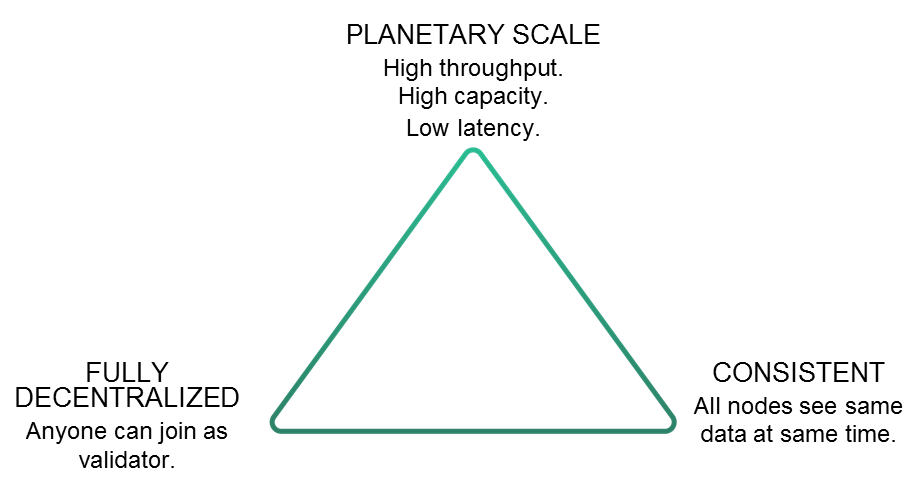
\includegraphics[width=\linewidth]{images/dcs-triangle.png}
    \caption{DCS Triangle}
    \label{fig:dcs_triangle}
\end{figure}

Per la communitiy di Ethereum, ricercatori e sviluppatori, la scalabilità costituisce probabilmente la sfida principale da risolvere per permettere alle applicazioni basate sulla blockchain di raggiungere un adozione di massa. Attualmente esistono due percorsi principali che sono stati studiati per incrementare la scalabilità delle blockchain. Da un lato si cerca di costruire dei protocolli al di sopra della blockchain base (chiamati *protocolli di livello 2*) senza cambiarne la struttura, che implicano l'invio di gran parte delle transazioni su catene secondarie. Dall'altro lato si cercano soluzioni che migliorino il design della blockchain di base, e una possibile soluzione da questo punto di vista è lo *sharding*.

\subsection{Sharding}

Effettuare lo *sharding* (letteralmente *frammentazione*) della blockchain significa semplicemente partizionare la catena principale in catene più piccole e più veloci, rendendo il sistema complessivo più scalabile. Il modo per farlo sarebbe dividere lo stato e la storia delle transazioni sulla catena principale in partizioni più piccole chiamate *shard.* Ad esempio, uno schema di Sharding su Ethereum potrebbe realizzare uno shard per tutti gli indirizzi che iniziano con 0x00, uno per quelli che iniziano con 0x01 e così via. 

Nella forma più semplice di sharding, ciascuno shard ha la propria storia di transazioni, e l'effetto delle transazioni in uno shard ha un effetto solo sullo shard stesso. In forme più avanzate di sharding esiste una qualche forma di comunicazione tra uno shard e l'altro (*cross-shard*), dove una transazione all'interno di uno shard può generare eventi all'interno di altri shard.

Realizzare lo sharding eliminerebbe la necessità che ciascun nodo processi ogni singola transazione all'interno della rete, dovendosi occupare soltanto di un sottoinsieme delle transazioni dell'intero sistema.

Oltre alle ricerce svolte per migliorare la scalabilità di Ethereum, che ha rilasciato una *roadmap* che dovrebbe portare allo sharding, esiste un progetto interessante con l'obiettivo di pubblicare un nuovo registro distribuito che superi i limiti di scalabilità di blockchain come Bitcoin ed Ethereum.

\section{Radix DLT}

Radix DLT è una nuova piattaforma simile a Bitcoin o Ethereum, ma realizzato con l'obiettivo di essere scalabile. I suoi creatori, invece di utilizzare la blockchain, sono partiti con un design completamente nuovo.

Radix utilizza un nuovo algoritmo di consenso chiamato Cerberus, basato su un *three-phase commit* e sullo *sharding,* per creare un sistema sicuro e scalabile. Attualmente, il progetto (diventato recentemente *open-source*) è ancora in fase di sviluppo, e non è ancora disponibile una rete pubblica.

\subsection{Un po' di storia}

La storia di Radix inizia nel 2013, quando il suo creatore, Dan Hughes, iniziò ad eseguire una serie di test per verificare quali fossero i limiti della scalabilità di Bitcoin. Il massimo che riuscì ad ottenere da questi test fu un numero di transazioni per secondo (*Transactions Per Second* o *TPS*) fra 700 e 1,000. Si tratta di cifre molto basse, sapendo che, ad esempio, Visa era in grado di processare circa 24,000 TPS. 

Dan, da questo punto in poi, tentò di percorrere diverse strade per aumentare il throughput di transazioni, talvolta riuscendoci, a scapito però della sicurezza. Dopo alcuni tentativi infruttuosi, Dan teorizzò ciò che divenne il primo nucleo di Radix, ovvero il *ledger* Tempo. Tempo ha una struttura basata sullo sharding, che raggruppa fra di loro le transazioni correlate e separa quelle non correlate, ed utilizza un meccanismo di consenso basato sui *Logical Clock* di Lesie Lamport (un meccanismo semplice per costruire un ordine parziale e relativo degli eventi). Dan iniziò quindi a cercare membri per formare un team, che iniziò a lavorare su Tempo, sulla costruzione della rete Radix e sul Radix Engine, cioè il livello applicativo di Radix (in sostanza, la parte con la quale interagiscono gli sviluppatori). 

\subsection{Un milione di transazioni al secondo}

Tutto questo lavoro portò a compiere un test facendo passare l'intera storia di transazioni di Bitcoin sul regstro Tempo, durante il quale il sistema raggiunse la velocità di 1M di TPS Questo fu certamente un grosso traguardo per Dan e il suo team, dimostrando l'enorme scalabilità ottenibile grazie a Tempo. Tuttavia, in seguito emersero delle vulnerabilità che esponevano Tempo a due possibili vettori di attacco. Il primo è quello che gli sviluppatori di Radix chiamano "*Weak Atom Problem"*, una situazione in cui un piccolo gruppo di nodi può creare una situazione in cui il consenso è sufficientemente debole da permettere di influenzare transazioni già concluse. Il secondo vettore di attacco era invece attraverso un attacco *Sybil.* Tempo infatti usava un nuovo meccanismo per proteggersi da questo tipo di attacco, chiamato *Mass*, che aumentava la reputazione dei nodi all'interno della rete per la loro buona condotta nel corso del tempo. Tuttavia, è emerso che Mass non avesse grande valore per gli attori "onesti", e questo apriva la strada ad un possibile mercato secondario, dove attori malevoli avrebbero potuto acquistare reputazione  (attraverso Mass) per un valore inferiore al vero.

Nonostante tutti quanti si rimboccarono le maniche e cercarono in tutti i modi di risolvere questi problemi, nessuna soluzione valida venne trovata, per cui, a malincuore, Dan e il suo team furono costretti a mettere da parte Tempo, e ad annullare il rilascio della rete pubblica Radix, previsto inizialmente per la fine del 2019.

\subsection{Cerberus}

Al momento della scrittura di questa tesi (Febbraio 2020), il team è al lavoro su un nuovo algoritmo di consenso, chiamato *Cerberus*. Cerberus utilizza il concetto di uno *shard space* predefinito usato da Tempo, ma al tempo stesso si basa su una serie di strumenti crittografici ben collaudati, che gli forniscono forti garanzie per quanto concerne la sicurezza. Attualmente, di Cerberus sappiamo che utilizza un meccanismo di consenso *BFT* (*Byzantine Fault Tolerant*) e *three-phase commit,* e che utilizzerà la Proof-of-Stake (PoS) come meccanismo di guardia contro attacchi *Sybil*. Il whitepaper di Cerberus è stato pubblicato in data 3 marzo 2020, durante le fasi finali di stesura della tesi. Il poco tempo a disposizione non mi ha purtroppo permesso di approfondire meglio Cerberus.

All'inizio del 2020 il team ha deciso anche di rendere *open-source* il progetto Radix, per rendere più partecipe la community sui progressi degli sviluppatori, oltre che dare la possibilità a chiunque di contribuire.

\subsection{Strumenti per gli sviluppatori}

Radix DLT offre agli sviluppatori interessati a creare applicazioni che interagiscano con il registro distribuito di Radix due librerie: una libreria Java e una libreria JavaScript, entrambe ancora in versione beta. Non essendovi una rete pubblica, per testare le librerie è necessario comunicare con la rete di testing *BETANET,* che può essere anche emulata in ambiente locale. Per questa tesi ho deciso di utilizzare la libreria JavaScript per realizzare una piccola applicazione che presenterò nei prossimi capitoli.

\subsection{Libreria JavaScript}

La libreria JavaScript Radix è costruita per essere eseguita sia client side che server side. E' costruita interamente utilizzando TypeScript, permettendo agli sviluppatori di costruire applicazioni più robuste sfruttando il *type checkin.* Inoltre, tale libreria segue il paradigma *reactive programming*, e si appoggia alla libreria RxJS.

\subsubsection{Concetti fondamentali}

Le librerie di Radix si basano su una serie di astrazioni, raggruppate in un modello chiamato *atom model*. I concetti fondamentali sono i seguenti:
\begin{itemize}
    \item \textit{Universe}: Il concetto di *Universe* rappresenta la rete Radix. Attualmente sono disponibili diversi Universe di testing ai quali connettersi. Essendo Radix basato sullo sharding, ciascun Universe è segmentato in un certo numero di *shards.* 
    \item \textit{Atom}: Un *Atom* rappresenta tutti gli eventi che si verificano all'interno di un Universe, e che hanno l'effetto di lo stato del registro. Ciascun atom contiene al suo interno almeno un *enpoint address* di destinazione.
    \item \textit{Address}: Un *Address* risiede su un particolare Shard, e costituisce punto di partenza e punto di arrivo per qualunque Atom nel Radix Universe. Si tratta di un riferimento ad un particolare Account, e permette ad un utente di ricevere fondi e/o dati sulla rete ad altri utenti. Gli indirizzi Radix vengono generati partendo da una chiave pubblica e da un checksum dell'Universe. 
    \item \textit{Account}: Un *Account* rappresenta tutti i dati salvati sul *ledger* per un particolare utente. Questi dati possono essere i token in possesso dell'utente, assieme ad altri dati arbitrari. Un account ha una serie di *account systems,* nei quali vengono salvati gli atom ricevuti dall'account. Gli account system di default sono:
    \begin{itemize}
        \item \textit{Il Transfer System}, che mantiene una lista delle transazioni in cui è coinvolto l'account, così come il saldo dell'account per tutti i differenti tipi di token.
        \item \textit{Il Radix Messaging System}, che gestire le diverse chat di messaggistica Radix a cui l'account partecipa.
        \item \textit{Il Data System}, usato per dati personalizzati salvati sul ledger.
        \item \textit{Token Definition System}, usato per gestire i token definiti dall'utente.
    \end{itemize}
    E' possibile accedere ai dati di questi sistemi attraverso l'utilizzo di mappe ES6, oppure è possibile effettuare il *subscribe* ad un *subject* RxJS, che emetterà un aggiornamento ogni volta che un sistema riceve un nuovo atom dalla rete.
    \item \textit{Identity}: Un'*identity* è una chiave privata associata ad un certo account, che può essere usata per firmare atom e per leggere dati criptati.
    \item \textit{Transaction Builder}: Il *Transaction builder* è il componente della libreria che si occupa di creare ed inviare alla rete qualsiasi tipo di Atom che il ledger radix possa accettare. Gli Atom che si possono creare con il transaction builder sono:
    \begin{itemize}
        \item \textit{Transfer Atom}: realizza il trasferimento di un item (e.g. valuta) ad un certo indirizzo.
        \item \textit{Payload Atom}: contiene dati inviati ad uno o più indirizzi.
        \item \textit{Radix Message Atom}: contiene un messaggio (caso particolare di payload atom).
        \item \textit{Mint Atom}: effettua il *minting* (cioè la creazione) di una quantità specificata di token.
        \item \textit{Burn Atom}: effettua il *burning* (cioè, in sostanza, l'eliminazione) di una quantità specificata di token.
    \end{itemize}
\end{itemize}
Le librerie offrono anche le funzionalità necessarie per definire dei token personalizzati. I token definiti dall'utente possono essere *single-issuance* o *multi-issuance*: i token *multi-issuance*, di cui si può fare il minting dopo la creazione, mentre i token *single-issuance* sono limitati all'importo specificato nella definizione del token.

\subsubsection{Radix Wallet}

Radix offre anche il software Desktop Wallet, un'applicazione che l'utente può utilizzare per memorizzare la propria identity. Il Wallet inoltre offre all'utente un interfaccia da cui:è
\begin{itemize}
    \item Controllare il saldo del proprio account.
    \item Inviare token ad un altro account.
    \item Avviare una chat di messaggistica istantanea con un altro account.
    \item Richiedere token di test all'account Faucet.
\end{itemize}

\chapter{Presentazione dell'applicazione}

\section{Cosa voglio realizzare}
%‘‘’’
L'applicazione che ho deciso di realizzare prende ispirazione dal progetto open-source \textit{Shared Royalty Non-Fungible Token} (SRNFT), avviato dal Web3Studio, una organizzazione di Consensys che si occupa di R&S nel campo delle tecnologie Blockchain e delle DApp. Lo scopo di tale progetto è quello di rendere qualunque sistema di Royalty, dall'industria del gas e del petrolio, fino all'intrattenimento, gestibile attraverso la blockchain Ethereum. Tale progetto si basa sul Token SRNFT che si presenta come una estensione del Token ERC721, ed offre tre funzionalità principali:
\begin{enumerate}
    \item Gestire e distribuire cash flow futuri verso destinatari multipli, chiamati Franchisors.
    \item Rendere unici e tracciabili asset digitali off-chain.
    \item Creare incentivi per i proprietari di tali asset affinché non li diffondano in maniera impropria al pubblico.
\end{enumerate}
Il SRNFT mantiene una lista di account Ethereum chiamati ‘‘franchisors’’ nella forma di un array, in maniera che un singolo token possa gestire cash flow verso parti multiple, in base ad una formula di distribuzione di royalties (\textit{Royalty Distribution Formula} o RDF). La RDF implementata può variare in base a quelli che sono gli incentivi che si vogliono creare nei diversi casi d'uso.

Vediamo come nell'implementazione di Web3Studio, il contratto per ciascun token SRNFT mantenga una semplice struttura dati (Fonte: \href{https://github.com/ConsenSys/web3studio-bootleg/blob/master/packages/bootleg-tokens/contracts/AbstractSharedRoyaltyToken.sol#L13}{AbstractSharedRoyaltyToken.sol}):

\begin{lstlisting}[language=Solidity,numbers=none]
struct Token {
  // The list of franchisors
  address[] franchisors;

  // A list of payments (in wei). Payment indices line up to
  // what payment was made for the matching franchisor
  uint256[] payments;

  // For any franchisor, what is the next payment index that a
  // withdrawal should next consider.
  // (More details on this part later.)
  mapping(address => uint256) franchisorNextWithdrawIndex;
}
\end{lstlisting}

Ogni volta che viene aggiunto un nuovo Franchisor, solitamente quando un token viene trasferito da proprietario all'altro, vengono effettuate alcune operazioni:

\begin{lstlisting}[language=Solidity,numbers=none]
function _addFranchisor (
  address franchisor, uint256 payment, uint256 tokenId)
{
  // A new franchisor is added to the list
  token.franchisors.push(franchisor);

  // Payments sent will be associated with that franchisor
  token.payments.push(msg.value);

  // We set where this franchisor can withdraw from
  token.franchisorNextWithdrawIndex[franchisor] = token.payments.length;
}
\end{lstlisting}

Un token ERC721 può avere un solo proprietario, e questa restrizione viene mantenuta nel SRNFT (gli stessi autori del progetto specificano che sarebbe interessante modificare tale aspetto, in modo da avere account multipli come proprietari del token). Dunque, nonostante vi possano essere più franchisor, solo quello aggiunto più recentemente ha la possibilità di trasferire il token ad un nuovo proprietario.

Il Web3Studio presenta come caso d'uso per questo token, un'applicazione specifica per il campo dell'industria musicale, chiamata \textit{Bootleg}, che ho utilizzato come spunto per l'applicazione da realizzare.

\subsection{L'applicazione radix-bootleg}
Ispirandomi dunque all'applicazione ‘‘fittizia’’ Bootleg di Web3Studio, ho deciso di realizzare una mia versione di questo progetto, che fosse però basata sulla libreria JavaScript di Radix DLT. 

L'idea di base dell'applicazione, è quella di consentire ai musicisti di costruire una nuova fonte di guadagno basata sulla distribuzione dei bootleg, ovvero le registrazioni degli spettacoli dal vivo realizzate dai fan (cosiddetti \textit{bootlegger}). Mentre tradizionalmente i bootleg si diffondono in maniera non ufficiale[riferimento], in questo caso di artisti ricevono royalties dalla vendita dei bootleg che condividono con i bootlegger. Inoltre, anche i fan che acquistano un bootleg, hanno la possibilità di condividere con l'artista le royalties generate da vendite future di tale contenuto. Questo costituisce un incentivo per i fan a non copiare il video e a diffonderlo in maniera indipendente, ad esempio attraverso altri canali non ufficiali (come ad esempio BitTorrent). Si presume comunque che i bootlegger siano in qualche modo autorizzati alla registrazione, in modo più o meno professionale, del concerto dell'artista. Tuttavia, questo discorso è al di fuori dello scopo di questa tesi.

L'applicazione permette ai bootlegger di caricare i bootleg inserendo tutte le informazioni necessarie e di metterli così a disposizione degli altri utenti. Così come nell'applicazione per Ethereum, il bootleg viene rappresentato da un token univoco. Chi accede all'applicazione, ha la possibilità di visualizzare un elenco dei Bootleg disponibili e di acquistarli. Una volta acquistato un bootleg, il pagamento viene inizialmente diviso fra il bootlegger e l'artista. L'utente che acquista un bootleg riceve così il token univoco per quel bootleg, e ottiene la possibilità di visionare liberamente la registrazione del concerto. Dopo l'acquisto, l'utente viene aggiunto alla lista dei franchisor, e in quanto tale condividerà con artista e bootlegger le royalties generate dai futuri acquisti del bootleg da parte di altri utenti.

\section{Architettura dell'applicazione}

Radix Bootleg è un applicazione strutturata principalmente in due parti: Il Frontend e il Bootleg Service. Il Frontend è la parte che si interfaccia con l'utente, e comunica con il Bootleg Service per svolgere le funzionalità relative ai token bootleg e ai pagamenti. Il Bootleg Service in sostanza implementa le funzionalità che, in una DApp per Ethereum, sarebbero realizzate con uno Smart Contract.

\subsection{Bootleg Service}

Il Bootleg Service ha le seguenti funzionalità:
\begin{itemize}
    \item Creazione del token nativo dell'applicazione, il BTLG.
    \item Creazione del token univoco per il bootleg.
    \item Salvataggio su database delle informazioni relative al bootleg.
    \item Divisione del pagamento per un bootleg tra Artista, Bootlegger ed eventuali franchisors, sulla base di una Royalty Distribution Formula (RDF).
    \item Fornire agli utenti la lista dei bootleg presenti nell'applicazione.
    \item Consente ai franchisor di visualizzare i bootleg che hanno acquistato, inviando l'url della registrazione su richiesta.
\end{itemize}

Il Bootleg service dunque si interfaccia sia con il Frontend che con il database dell'applicazione. Il database ha lo scopo di mantenere i ‘‘metadati’’ del bootleg token, ovvero: titolo, descrizione, URL del contenuto, nonché gli indirizzi di artista, bootlegger e franchisors, in maniera tale da sapere chi sono i destinatari delle royalties generate da un particolare bootleg. Il Bootleg Service ha inoltre il compito di verificare che un franchisor, nel momento in cui richiede di visualizzare un bootleg, possieda effettivamente il token per quel bootleg.

\subsection{Front End}

Il front-end invece realizza l'interfaccia utente dell'applicazione, ed offre le seguenti funzionalità:
\begin{itemize}
    \item Consente ai franchisor di visualizzare i bootleg che hanno acquistato.
    \item Autenticarsi attraverso il Radix Wallet.
    \item Accedere alla lista dei bootleg disponibili e quelli acquistati.
    \item Visionare i bootleg acquistati.
    \item Visualizzare il saldo dell'account.
    \item Visualizzare le transazioni dell'account.
\end{itemize}

Il front-end comunica con il Bootleg Service per ricevere le informazioni sui bootleg presenti nel sistema, nonché per l'invio dei pagamenti e della divisione di questi tra i diversi destinatari.

\chapter{Implementazione}
%‘‘’’
Sia per la realizzazione del front end che del discovery service ho utilizzato TypeScript, sfruttando le funzionalità offerte dalla libreria JavaScript di Radix. 

Per velocizzare lo sviluppo del discovery service, ho usato come base di partenza un server realizzato con TypeScript e WebPack. Ad esso ho aggiunto il codice per la connessione ad un database locale MongoDB, per tenere traccia di tutte le informazioni relative ai bootleg. Essendo a tutti gli effetti un server, per comunicare con il Discovery Service vengono utilizzate delle normali richieste http, costruite utilizzando la libreria axios.

Per il front end invece ho utilizzato il framework Vue.js, in quanto permette di realizzare un interfaccia utente in maniera piuttosto semplice, e inoltre consente di mantenere le astrazioni di Radix (Atom, Transazioni, ecc.) separate dal codice HTML.

Come già accennato in precedenza, attualmente non è stata ancora attivata la rete pubblica di Radix, dunque per sviluppare applicazioni è necessario simulare la rete sulla propria macchina. Per farlo, è disponibile un emulatore da eseguire in locale, attraverso un'immagine Docker. Una volta lanciato l'Emulator, sarà disponibile collegarsi ad una rete Radix ed eseguire correttamente l'applicazione. Il modo in cui eseguire il Betanet Emulator sulla propria macchina è spiegato nella documentazione di Radix: [https://docs.radixdlt.com/kb/develop/betanet-emulator](https://docs.radixdlt.com/kb/develop/betanet-emulator). 

Sempre nella documentazione Radix è possibile consultare diversi esempi di codice che sono stati fondamentali durante l'implementazione del progetto.

\section{Utilizzo dei Token}

Per effettuare i pagamenti dei bootleg all'interno dell'applicazione, viene usato il token BTLG. Il discovery service definisce il token BTLG al suo primo avvio come un token multi-issuance. Nel momento in cui un utente crea una nuova identity, il frontend invia una richiesta al discovery service per ricevere una somma iniziale di token BTLG token. In sostanza, il Discovery Service prende il posto del Faucet, ovvero un account particolare che ha lo scopo di inviare dei token nativi di test. 

Il Discovery Service ha anche il compito di definire un Token univoco per ciascun bootleg nel momento della sua creazione. Il possesso di questo Token da parte di un utente è ciò che indica al sistema che tale utente ha acquistato il relativo bootleg, e pertanto è autorizzato a visualizzarlo.

\section{Gestione dell'identity}

La libreria Radix offre delle funzionalità per la gestione delle identity all'interno di un'applicazione. La funzione `encryptKey`, date in input un'identity e una password, cifra la prima producendo in output un oggetto JSON detto anche \textit{keystore}. L'identity viene decifrata usando la funzione `decryptKey`, fornendo in input il keystore e la password utilizzata per produrlo.

Per la gestione dell'identity all'interno dell'applicazione sono disponibili due diverse opzioni:
\begin{itemize}
    \item Generare una nuova identity locale.
    \item Usare un'identity remota.
\end{itemize}

\begin{figure}[H]
  \centering
  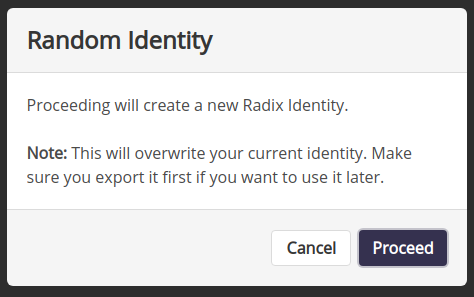
\includegraphics[width=0.75\textwidth]{images/application/create_random.png}
  \caption{Creazione di una nuova identity locale}
  \label{fig:trex}
\end{figure}

Quando l'utente genera una nuova identity locale, questa viene automaticamente cifrata con una password di default e il keystore viene salvato nella memoria del browser utilizzando la proprietà `Window.localStorage`. In questo modo, l'identity viene recuperata all'avvio successivo del browser. Quando l'utente genera una nuova identity locale, quella precedente viene sovrascritta. Tuttavia, l'applicazione offre anche la possibilità di \textit{esportare} la propria identity: Facendo export l'applicazione chiede all'utente di inserire una password per cifrare la chiave, e mostra il keystore JSON prodotto. L'utente può così salvare il contenuto del keystore all'interno di un file, che potrà così essere recuperato in un secondo momento. Con la funzione *import* infatti, l'utente inserisce il *keystore* e la password inserita in precedenza, e l'identity che ha esportato viene così importata dentro l'applicazione.

\begin{figure}[H]
  \centering
  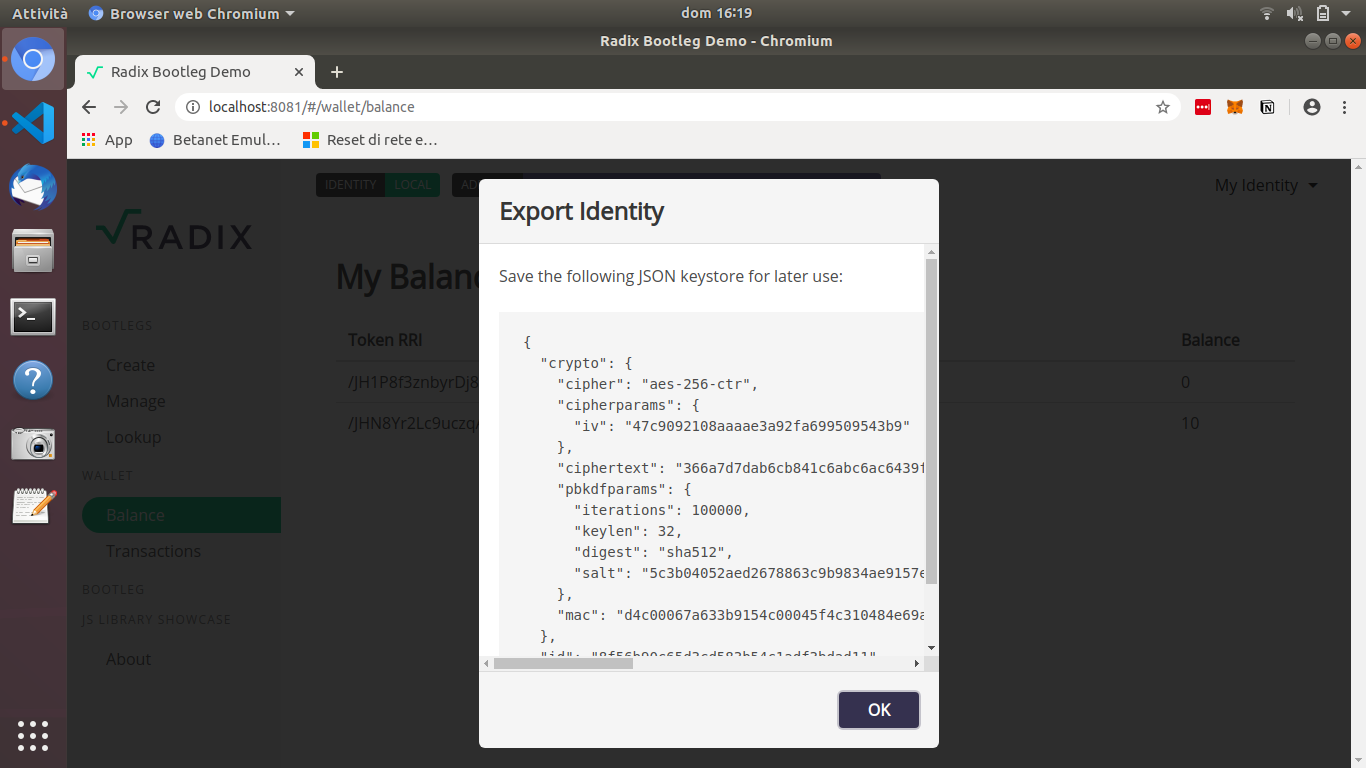
\includegraphics[width=\linewidth]{images/application/save-keystore.png}
  \caption{Esportazione di un'identity locale}
  \label{fig:trex}
\end{figure}

Usando un'identity remota invece, l'applicazione userà la chiave privata salvata nel Radix Wallet dell'utente, che pertanto non necessita di essere salvata nel browser. In questo caso, l'applicazione invia una richiesta al Radix Wallet. Una volta che l'utente accetta la richiesta, l'applicazione potrà usare la chiave privata mantenuta nel Wallet per firmare atom per conto dell'utente. 

\section{Creazione di un bootleg}

Per creare un bootleg, è necessario inserire:
\begin{itemize}
    \item Simbolo usato per il token;
    \item Titolo del bootleg;
    \item Indirizzo dell'artista;
    \item Prezzo del bootleg;
    \item Url del bootleg (Per semplicità sono stati utilizzati dei link di video su YouTube);
\end{itemize}

Quando l'utente da la conferma, questi vengono inviati al server (Discovery Service), che provvederà a creare il token per il bootleg e salverà tutti i dati inviati dall'utente sul database, insieme all'identificativo del token appena creato, ed agli indirizzi di bootlegger e artista. Terminato l'inserimento, il Discovery Service invierà all'utente l'identificativo del token come conferma.

\section{Acquisto di un bootleg}

L'applicazione recupera la lista dei bootleg inseriti sul database inviando una richiesta al Discovery Service, che esegue una query e recupera tutti i dati dei bootleg (ad eccezione dell'url del video), e li invia al frontend.

Per ciascun bootleg nella lista, il front end verifica se sono presenti nell'account dell'utente, e in caso contrario mostra un pulsante ‘‘Buy’’.

Quando un utente acquista un bootleg, l'applicazione verifica che il suo account possieda un ammontare sufficiente di BTLG. Se si, il pagamento viene inviato al discovery service, insieme ai dati del bootleg da acquistare. Il Discovery Service può così dividere il pagamento in parti uguali tra artista, bootlegger ed eventuali franchisor.

Una volta che il pagamento è stato diviso tra i vari destinatari, il discovery service procede con l'invio del token all'utente ed inserisce quest'ultimo nella lista dei franchisor per quel token, aggiornando i dati sul database. In questo modo, quando verrà effettuato un nuovo acquisto del bootleg, l'utente riceverà una percentuale del pagamento come franchisor. 

\section{Visualizzazione del bootleg}

Una volta che l'utente possiede il token, nella lista dei bootleg compare il pulsante ‘‘Watch’’ di fianco al bootleg, che consente all'utente di visualizzare il bootleg. Dal momento che il front-end non possiede di per se l'url del video, deve richiederlo al Discovery Service. Il modo in cui il frontend richiede ed ottiene il link al contenuto del bootleg si basa su uno schema challenge-response. 

Cliccando su ‘‘Watch’’ il front end invia una richiesta al Discovery service per il link al bootleg.Quando il DS riceve questa richiesta, crea una \textit{challenge} casuale, la salva nel database insieme ad un attributo boolean \textit{consumed}, inizialmente settato a ‘‘false’’, per indicare che la challenge non è stata ancora utilizzata per accedere ad un bootleg. 

Quando il frontend riceve la challenge dal Discovery Service, crea un nuovo Payload Atom contenente la challenge, firma questo Atom con la propria identity e lo invia al Discovery Service con una richiesta http insieme all'URI del token del bootleg da visualizzare.

Una volta che il Discovery Service riceve anche questa richiesta:
\begin{enumerate}
    \item Estrae l'atom dalla richiesta e verifica la validità della firma dell'atom, cioè controlla se è stata prodotta dall'account che ha creato l'atom. Se la firma viene verificata con successo, il DS procede con la verifica della challenge.
    \item Verifica la validità della challenge: il DS estrae la challenge dal payload dell'atom, ed esegue una query sul database per trovare la challenge ricevuta. Se non viene trovata la challenge, oppure viene trovata ma l'attributo ‘‘consumed’’ ha valore ‘‘true’’ (dunque è già stata utilizzata), la challenge non viene considerata valida e il DS restituisce un errore al frontend. Altrimenti, aggiorna il valore di ‘‘consumed’’ a true sul database e prosegue al passo successivo.
    \item Verifica il possesso del bootleg: Il DS controlla il saldo dell'account dell'utente che ha inviato la richiesta e verifica se è presente il token del bootleg richiesto. Se il token è presente, allora il DS recupera il link del video dal database e lo invia come risposta al frontend.
\end{enumerate}

Una volta che il frontend riceve il link del bootleg, mostra all'utente il video YouTube attraverso un elemento `<iframe>`.


%%%%%%%%%%%%%%%%%%%%%%%%%%%%%%%%%%%%%%%%%per fare le conclusioni
\chapter*{Conclusioni}
%%%%%%%%%%%%%%%%%%%%%%%%%%%%%%%%%%%%%%%%%imposta l'intestazione di pagina
\rhead[\fancyplain{}{\bfseries
CONCLUSIONI}]{\fancyplain{}{\bfseries\thepage}}
\lhead[\fancyplain{}{\bfseries\thepage}]{\fancyplain{}{\bfseries
CONCLUSIONI}}
%%%%%%%%%%%%%%%%%%%%%%%%%%%%%%%%%%%%%%%%%aggiunge la voce Conclusioni
                                        %   nell'indice
\addcontentsline{toc}{chapter}{Conclusioni} 

In conclusione, in questa tesi è stata esposta una panoramica generale sulle blockhain, sulla loro storia e sulle caratteristiche principali di questa tecnologia, esponendo i casi di Bitcoin ed Ethereum, rispettivamente la prima e la seconda tra le criptovalute con maggior capitalizzazione di mercato. Si è visto poi come questa tecnologia, fornendo sicurezza e di consenso su di un unico ordine degli eventi in una rete distribuita senza bisogno di un'autorità centrale, abbia visto espandere i suoi possibili utilizzi. Dalle criptovalute, si è passati ad avere possibili applicazioni nei campi più disparati.
Partendo da questa base, è stato esposto il problema della scalabilità delle blockchain, e di quali sono state alcune fra le soluzioni proposte, in particolar modo, lo \textit{sharding}. Dunque è stata presentata una nuova tecnologia DLT, ovvero Radix. Essa si presenta come una piattaforma alternativa alle blockchain, ma caratterizzata da scalabilità e facilità nel costruire applicazioni che sfruttino il suo registro distribuito come base. Dopo aver visto come Radix riesce ad essere scalabile, per verificare con mano la facilità nella costruzione di applicazioni, è stata implementata un'applicazione utilizzando la libreria JavaScript di Radix. 

\subsubsection{Implementazione}

Durante l'implementazione di tale applicazione, si è effettivamente riscontrato come la presenza di librerie che utilizzano linguaggi altamente diffusi consenta ad uno sviluppatore di implementare facilmente applicazione basate sul ledger Radix. Le difficoltà riscontrate durante lo sviluppo certamente includono una documentazione che forse a volte non è abbastanza dettagliata, e l'assenza di una community di sviluppatori folta ed attiva attorno alla piattaforma Radix. La causa di ciò è probabilmente da ricercare nel fatto che si tratta ancora di un progetto in via di sviluppo. Tuttavia, i canali di comunicazione presenti (principalmente Telegram e Discord) sono stati utili per ricevere supporto durante la fase di implementazione.

\subsubsection{Limiti dello stato attuale}

Uno dei limiti dello stato attuale di Radix è certamente quello di non avere ancora a disposizione una rete pubblica stabile e robusta, nonché la necessità di dover simulare una rete in locale per poter testare le proprie applicazioni. Attualmente, non si sa ancora quando la rete pubblica di Radix sarà disponibile. Il suo rilascio è stato recentemente posticipato a causa di problemi di sicurezza che hanno portato gli sviluppatori a cambiare l'algoritmo di consenso alla base del ledger Radix, non senza generare qualche scetticismo da parte della community esistente intorno al progetto. Questo probabilmente anche per il fatto che, nonostante diversi canali di comunicazione disponibili (fra cui Telegram e Discord), si ha come membri della communitiy la sensazione di non avere veramente un idea chiara al 100\% su ciò che succede dietro le quinte. Certamente la scelta di rendere il progetto open source \cite{K20} è stata effettuata anche con la volontà di maggiore trasparenza verso l'esterno, nonché per fornire la possibilità a soggetti esterni di dare il loro contributo al progetto.

\subsubsection{Possibili sviluppi futuri}

L'applicazione che è stata realizzata può fornire un esempio di ciò che è possibile realizzare utilizzando le librerie Radix, e dimostra come tali librerie possano essere facilmente integrate con un framework JavaScript, in questo caso Vue.js. Certamente si tratta di un'applicazione che potrebbe essere migliorata sotto molti aspetti. Alcuni sviluppi futuri dell'applicazione potrebbero includere:
\begin{itemize}
    \item Miglioramento della gestione del token nativo.
    \item Differenziare le funzionalità dell'applicazione disponibili per artista, bootlegger e franchisor.
    \item Consentire agli artisti di autorizzare il caricamento di un bootleg sulla piattaforma.
    \item La memorizzazione dei bootleg non più come video di YouTube, ma su un file system distribuito  (ad esempio IPFS: \cite{K30}).
\end{itemize}


\begin{thebibliography}{90}             %crea l'ambiente bibliografia
\rhead[\fancyplain{}{\bfseries
BIBLIOGRAFIA}]{\fancyplain{}{\bfseries\thepage}}
\lhead[\fancyplain{}{\bfseries\thepage}]{\fancyplain{}{\bfseries
BIBLIOGRAFIA}}
%%%%%%%%%%%%%%%%%%%%%%%%%%%%%%%%%%%%%%%%%aggiunge la voce Bibliografia
                                        %   nell'indice
\addcontentsline{toc}{chapter}{Bibliografia}

\bibitem{K1} S. Nakamoto, “Bitcoin: A Peer-to-Peer Electronic Cash System,” p. 9.
\bibitem{K2} A. M. Antonopoulos (2017, June). Mastering Bitcoin, Programming the open blockchain. O'Reilly Media.
\bibitem{K3} OECD, OECD Blockchain Primer.
\bibitem{K4} Consensys Academy. Blockchain Basics Book.
\bibitem{K5} District0x Education Portal, What Is An ERC20 Token?
\bibitem{K6} ERC721 Standard (2018) http://erc721.org/
\bibitem{K7} Consensys Web3Studio. Bootleg, A Community for Royalty Sharing. https://consensys.net/web3studio/bootleg.
\bibitem{K8} A. B. Bondi (2000), Characteristics of Scalability and Their Impact on Performance.
\bibitem{K9} L. Lamport (1978), Time, Clocks, and the Ordering of Events in a Distributed System.
\bibitem{K10} F. C{\"a}sar, D. P. Hughes, J. Primero, S. J. Thornton, Cerberus, A Parallelized BFT Consensus Protocol for Radix, v1.0 (2020, March).
\bibitem{K11} G. Minello (2019), Metodologie per la realizzazione di una Security Token Offering.
\bibitem{K12} Sophie Donkin (2020, February), Dan And Radix's Tech Journey. Radix DLT Blog. https://www.radixdlt.com/post/dan-and-radixs-tech-journey/
\bibitem{K13} Matthew Hine (2019, November), Radix Engine and Ledger: The Road to Adoption. Radix DLT Blog. https://www.radixdlt.com/post/radix-engine-and-ledger-the-road-to-adoption/
\bibitem{K14} Carlotta Balena, Liberi dagli intermediari. Fortune Italia n. 5, Maggio 2019, p. 60.
\bibitem{K15} Bootleg, Wikipedia.  https://it.wikipedia.org/wiki/Bootleg
\bibitem{K16} Ethereum GitHub Wiki (2019, April) Sharding FAQ.
\bibitem{K17} Trent McConaghy (2016), The DCS Triangle: Decentralized, Consistent, Scalable. Pick any two. Medium.
\bibitem{K18} The Radix Basics (2018) https://www.radixdlt.com/post/the-radix-basics/
\bibitem{K19} Radix Engine: A Simple, Secure Smart Contract Alternative (2019). https://www.radixdlt.com/post/radix-engine-a-simple-secure-smart-contract-alternative/
\bibitem{K20} Why we are open sourcing (2020). https://www.radixdlt.com/post/why-we-are-open-sourcing/
\bibitem{K21} Consensys Academy (2018, January), Ethereum Limitations and scaling solutions.
\bibitem{K22} Buterin, V. (2013). Ethereum white paper. GitHub repository
\bibitem{K23} Matthew Hine (2019) Radix Engine and Ledger, The road to adoption. Radix DLT Blog
\bibitem{K24} Radix Engine Library. radixdlt GitHub repository
\bibitem{K25} Axios Github Repository https://github.com/axios/axios
\bibitem{K26} https://radixdlt.github.io/library-api-docs/radixdlt-js/2.0.0-beta.1/
\bibitem{K27} https://docs.radixdlt.com/radixdlt-js/examples/code-examples
\bibitem{K28} https://github.com/radixdlt/radixdlt-js-showcase
\bibitem{K29} https://docs.radixdlt.com/kb/develop/betanet-emulator
\bibitem{K30} https://ipfs.io/

\end{thebibliography}

\end{document}
